We now examine the performance of our two new models (\emph{Instant}, \emph{Guarded}) as compared against existing RL work (\emph{Marl}) and {\color{revisiontext} \cbstart \emph{SPIFFY} under different traffic behaviour and topologies, varying the host-to-learner ratio $n$ and environment.
%?? Probably best just to look at top level stuff, and THEN a simplified comparison for each intended improvement (like banded rewards).
%Additionally, we examine the performance effects of environmental characteristics and potential improvements: negative reinforcement, the case where one agent makes all decisions, and pre-training on individual features.
We present the average rewards for all combinations of these factors in \crefrange{tab:av-vals}{tab:av-ecmp-vals}---providing a rough idea of expected performance, with the highest-performing model in bold and the best RL-based model \cbend underlined.}
Average rewards take into account any portions of time that an agent allows illegal system states.
Several plots augment this, illustrating peak performance or the amount of time which an agent requires to learn.

\begin{table}
	\centering
	\caption{Average reward for combinations of model, host density and traffic class with a single destination.\label{tab:av-vals}}
	
	\cbstart
	\resizebox{0.8\linewidth}{!}{
		\expandableinput tables/marl/tnsm-tree-avg-reward-spiffy.tex
	}
	\cbend
\vspace{-0.25cm}
\end{table}
\begin{table}
	\centering
	\caption{Average reward for combinations of model, host density and traffic class with multiple destinations.\label{tab:av-ecmp-vals}}
	
	\cbstart
	\resizebox{0.8\linewidth}{!}{
		\expandableinput tables/marl/tnsm-ecmp-avg-reward-spiffy.tex
	}
	\cbend
\vspace{-0.5cm}
\end{table}

\subsection{Congestion-unaware traffic}
%\begin{figure}
%	\centering
%	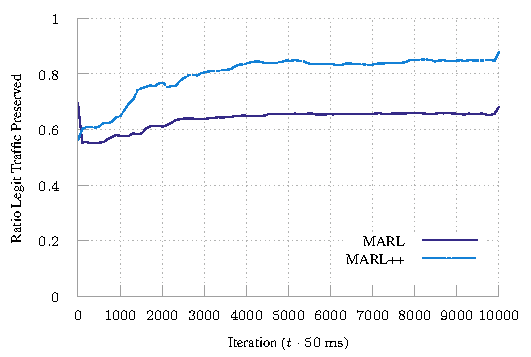
\includegraphics[width=0.9\linewidth]{../plots/udp-2}
%	
%	\caption{
%		Online performance for $n=2$ hosts per egress point when benign traffic is UDP-like.
%		Although Marl++ offers a marked improvement (a peak $\sim$\SI{30}{\percent} more benign traffic arrives unimpeded), SPF significantly underperforms for this relatively simple topology.
%		Non-SPF agents start off reasonably well, slowly learning better policies.
%		\label{fig:udp-2}
%	}
%\end{figure}
%\begin{figure}
%	\centering
%	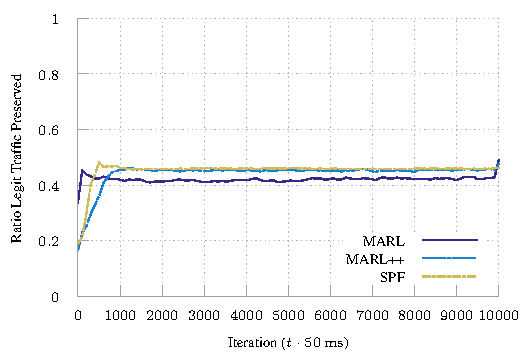
\includegraphics[width=0.9\linewidth]{../plots/udp-16}
%	
%	\caption{
%		Online performance for $n=16$ hosts per egress point when benign traffic is UDP-like.
%		Marl++ remains marginally ahead of its predecessor, though both have undergone a significant drop in effectiveness.
%		SPF, remarkably, displays performance on par with Marl++ for this more difficult topology.
%		Both of the new models take longer to train, but achieve better peak and average performance than Marl.
%		\label{fig:udp-16}
%	}
%\end{figure}
\begin{figure}
	\centering
	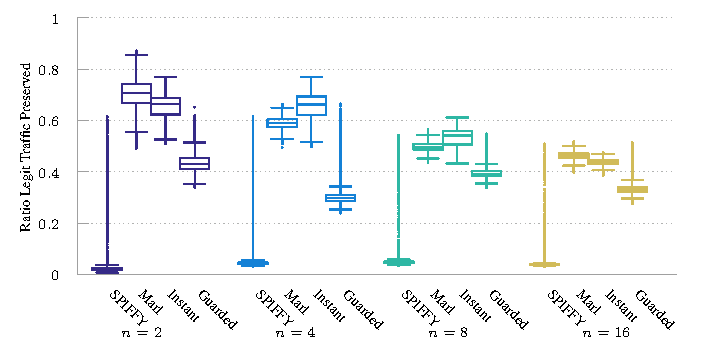
\includegraphics[width=0.75\linewidth]{plots/marl/tnsm-udp-box-separate}
	\vspace{-0.3cm}
	\caption{
		Online performance for Opus benign traffic in a single-destination network, multi-agent mode.
%		Marl++ offers a marked improvement (a peak $\sim$\SI{30}{\percent} more benign traffic arrives unimpeded) at small $n$, and remains marginally ahead of its predecessor by $n=16$, though both have undergone a significant drop in effectiveness.
		\emph{Instant} outperforms Marl for $n \in \{4, 8\}$ (with higher variance), but performs similarly to Marl at $n\in \{2, 16\}$.
		\emph{Guarded} underperforms compared to the other agent designs in this problem variant.
%		SPF, remarkably, slightly outperforms Marl++ (with lower variance) for this more difficult topology despite being worse for smaller $n$.
%		Both of the new models take longer to train, but achieve better peak and average performance than Marl.
%		?? REWORK/MAKE ACCURATE
		\label{fig:udp-tree-box}
	}
\vspace{-0.5cm}
\end{figure}

%\begin{figure}
%	\centering
%	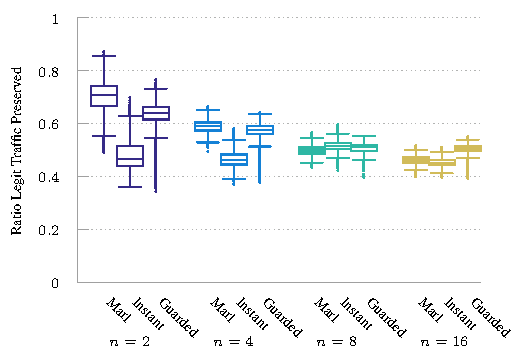
\includegraphics[width=0.95\linewidth]{../plots/tnsm-udp-box-single}
%	
%	\caption{
%		Online performance for Opus benign traffic in a single-destination network, single-agent mode.
%		?? DO I need this?
%		\label{fig:udp-tree-box-single}
%	}
%\end{figure}
%
%\begin{figure}
%	\centering
%	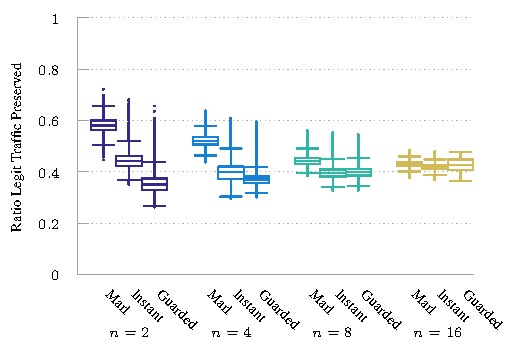
\includegraphics[width=0.95\linewidth]{../plots/tnsm-ecmp-udp-box-separate}
%	
%	\caption{
%		Online performance for Opus benign traffic in a multi-destination network, multi-agent mode.
%		?? DO I need this?
%		\label{fig:udp-ecmp-box}
%	}
%\end{figure}
%
%\begin{figure}
%	\centering
%	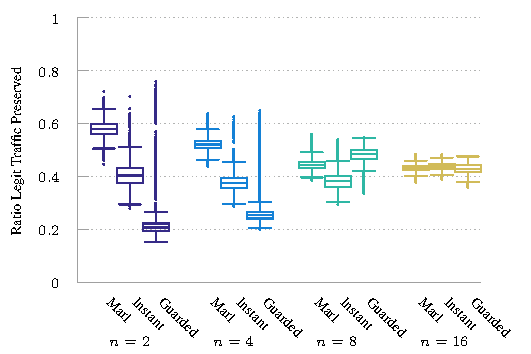
\includegraphics[width=0.95\linewidth]{../plots/tnsm-ecmp-udp-box-single}
%	
%	\caption{
%		Online performance for Opus benign traffic in a multi-destination network, single-agent mode.
%		?? DO I need this?
%		\label{fig:udp-ecmp-box-single}
%	}
%\end{figure}

In a single-destination network, we observe that Marl's performance degrades as $n$ increases.
Typically, our \emph{Instant} agent design achieves the best performance in multi-agent mode, having lower collateral damage than the current state-of-the-art, but sharply degrades at low $n$ when agents share experience.
This trend reverses for the \emph{Guarded} model, which improves as $n$ increases and in single-agent mode---when $n\ge4$, the single-agent variant offers consistent improvement.
%Across all choices of $n$, we see that Marl++ exhibits reduced collateral damage compared to Marl, with SPF starting poorly yet becoming more effective for larger $n$ (\cref{tab:av-vals}, \emph{Capped}, UDP).
\Cref{fig:udp-tree-box} shows the preserved traffic in multi-agent mode.
%?? Discuss multi-dest topol once all results available.
When defending multiple destinations, we see a sharp decrease in the effectiveness of all agent designs.
Our new agent designs become more effective as $n$ increases, while Marl's effectiveness is roughly constant (aside from the outlier at $n=12$).
Interestingly, SPIFFY is unable to effectively protect constant bitrate traffic.

\subsection{Congestion-aware traffic}
%\begin{figure}
%	\centering
%	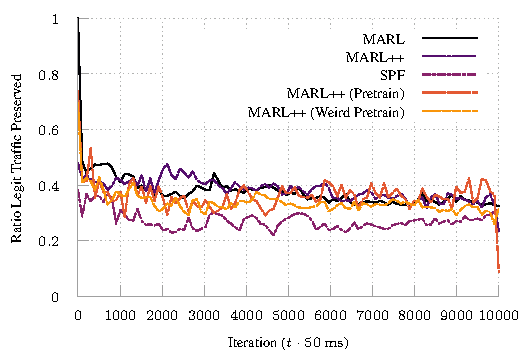
\includegraphics[width=0.9\linewidth]{../plots/tcp-2}
%	
%	\caption{
%		Online performance for $n=2$ hosts per egress point when benign traffic is TCP-like.
%		Marl++ and Marl achieve very similar performance, starting off similarly well without notable improvement over an episode.
%		SPF's performance is disappointingly close to baseline, indicating that it is as useful as having no defence system.
%		\label{fig:tcp-2}
%	}
%\end{figure}
\begin{figure}
%	\vspace{-0.5cm}
	\centering
	\includegraphics[width=0.75\linewidth]{plots/marl/tnsm-tcp-box-single}
	\vspace{-0.3cm}
	\caption{
		Online performance for HTTP benign traffic in a single-destination network, single-agent mode.
		\emph{Instant} and \emph{Guarded} exhibit similar efficacy at $n=2$, protecting less traffic than Marl.
		Only \emph{Guarded}'s performance rapidly increases with $n$, achieving a considerably better median and lower variance than the other models.
		The longer tails of outliers typically indicate the longer training time the new models require---we observe that \emph{Guarded} typically has considerably lower variance once it has converged on a stable policy.
		\label{fig:tcp-tree-box}
	}
\vspace{-0.6cm}
\end{figure}
%\begin{figure}
%	\centering
%	\includegraphics[width=0.95\linewidth]{../plots/tnsm-tcp-box-single}
%	
%	\caption{
%		Online performance for HTTP benign traffic in a single-destination network, single-agent mode.
%		?? DO I need this?
%		\label{fig-tcp-tree-box-single}
%	}
%\end{figure}
\begin{figure}
	\centering
	\vspace{-0.8cm}
	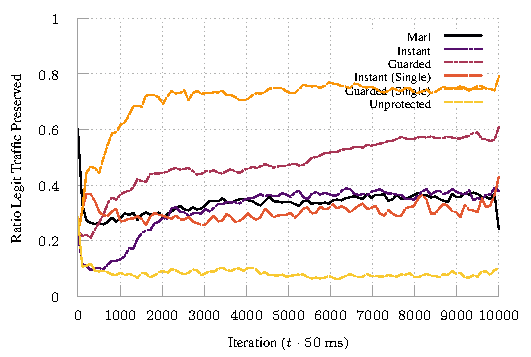
\includegraphics[width=0.75\linewidth]{plots/marl/tnsm-tcp-16-single}
	\vspace{-0.35cm}
	\caption{
		Online performance of standard and single-agent models in a single-destination network with $n=16$ hosts per egress point, HTTP traffic.
		At this level of host density, \emph{Guarded} reaches higher peak performance sooner and is considerably more consistent throughout the episode.
		\emph{Guarded} benefits greatly from information sharing, converging to protect around \SI{75}{\percent} of TCP traffic within \SI{100}{\second}.
		The \emph{Instant} model converges to Marl's level of performance.
%		With a single agent, Marl++ shows worse performance, while SPF improves significantly and continues to learn well past annealing $\epsilon \rightarrow 0$.
		\label{fig:tcp-tree-16}
	}
%\vspace{-0.5cm}
\end{figure}

%\begin{figure}
%	\centering
%	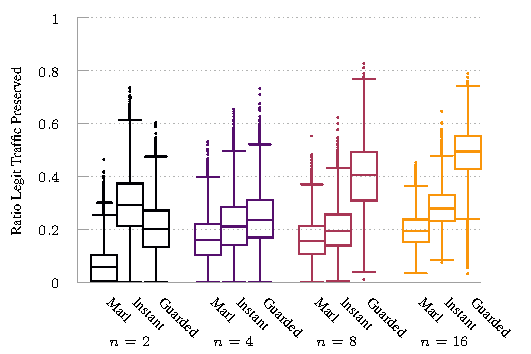
\includegraphics[width=0.95\linewidth]{../plots/tnsm-ecmp-tcp-box-separate}
%	
%	\caption{
%		Online performance for HTTP benign traffic in a multi-destination network, multi-agent mode.
%		?? DO I need this?
%		\label{fig:tcp-ecmp-box}
%	}
%\end{figure}

%\begin{figure}
%	\centering
%	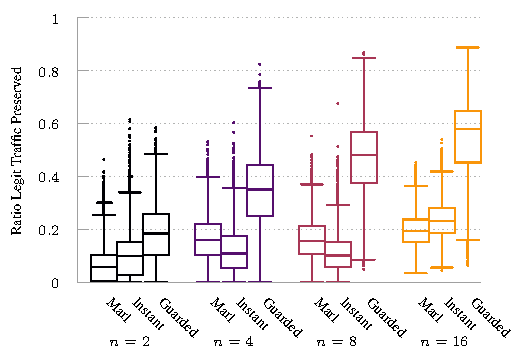
\includegraphics[width=0.95\linewidth]{../plots/tnsm-ecmp-tcp-box-single}
%	
%	\caption{
%		Online performance for HTTP benign traffic in a multi-destination network, single-agent mode.
%		?? DO I need this?
%		\label{fig:tcp-ecmp-box-single}
%	}
%\end{figure}

%\begin{figure}
%	\centering
%	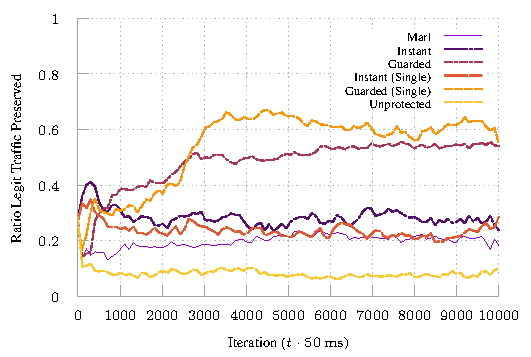
\includegraphics[width=0.95\linewidth]{../plots/tnsm-ecmp-tcp-16-single}
%	
%	\caption{
%		?? Eh
%		\label{fig:tcp-ecmp-16}
%	}
%\end{figure}

\Cref{tab:av-vals} shows that Marl offers a low (though fairly consistent) level of protection for TCP traffic, which the \emph{Instant} agent offers no substantial improvement over.
However, \emph{Guarded} agents offer a remarkable improvement for this class of traffic, particularly when experience can be shared---offering a \SI{2.21}{$\!\times$} improvement over the state-of-the art during training, which is made clearer in \cref{fig:tcp-tree-box}.
\Cref{fig:tcp-tree-16} shows that this model can protect a peak \SI{80}{\percent} of TCP traffic (\SI{2.5}{$\!\times$} improvement) after just \SI{100}{\second}, but also that all of the new models require considerably longer than Marl to learn their best-achieving policy.
%SPF reaches a stronger plateau before \emph{both}, remaining more consistent and appearing to continue learning.
%?? Discuss multi-dest topol once results available.
We observe that the same trends present themselves in the multi-destination topology: \emph{Guarded} remains the best fit for TCP, in both training modes.
Crucially, the rigid tree of learners and teams which define Marl, along with its lack of action granularity, seem to be a poor fit in this environment.
{\color{revisiontext}In both cases, SPIFFY greatly outperforms the RL-based methods.}

%\subsection{Single-agent performance}
%Making all decisions with a single agent is roughly equivalent to having a zero-cost communication channel between each pair of agents, theoretically allowing faster training by giving each agent more experience.
%Curiously, we observe that this often leads to drastically worse policies when used as part of Marl++ for small $n$, but makes SPF a considerably more competitive model---especially for TCP, and as $n$ grows larger (\cref{fig:tcp-16}).
%Single-agent SPF almost consistently outperforms Marl.
%We discuss our conjectures for why this reversal occurs in \cref{sec:discussion}.

\subsection{Increased Attack Volume}\label{sec:results-attack-volume}
To assess the effect of larger volumes of attack traffic, we increase an attacker's output by various factors, supposing $n=16$ with HTTP traffic (\emph{Guarded}, Single); \cref{tab:atk-vol} records the expected rate of attack and average performance.
The initial increase in traffic volume causes the steepest reduction in performance (due to the increased cost of incorrect action), though performance levels out as attack traffic increases.

\begin{table}
	\centering
%	\vspace{-0.1cm}
	\caption{Average reward versus attack volume.\label{tab:atk-vol}}
\resizebox{0.45\linewidth}{!}{
\begin{tabular}{@{}SSS@{}}
	\toprule\multicolumn{1}{c}{Factor} & \multicolumn{1}{c}{$\mathbb{E}\left[V_{\mathit{attack}}\right]$ (\si{\mega\bit\per\second})} & \multicolumn{1}{c}{Reward} \\ \midrule
	1.5 & 633.6 & 0.671 \\
	2.0 & 844.8 & 0.625 \\
	2.5 & 1056.0 & 0.620 \\
	3.0 & 1267.2 & 0.619 \\
	3.5 & 1478.4 & 0.600 \\
	\bottomrule
\end{tabular}
}
\vspace{-0.75cm}
\end{table}

\subsection{Computational Cost}
%?? Consider talking about the execution times of the old MARL approach here? They're real nice (as expected), so we have lots of room to play around with while (hopefully) remaining under the 1ms target time given by \textcite{DBLP:conf/sigcomm/ChenL0L18}.

%Overall, each episode takes around \SI{10}{\minute} to run, while each set of \num{10} requires around \SI{2}{\hour} due to additional set-up/tear-down costs associated with mininet.
Measurements from each of these experiments indicated that the cost of computing any action is typically within \SIrange{80}{100}{\micro\second} per flow.
This is reassuring when measured alongside the insights from other work.
\Textcite{DBLP:conf/sigcomm/ChenL0L18} observe that, ideally, actions must be computed and taken within \SI{1}{\milli\second} to have a meaningful affect on short flows.
%Most flows are short, and flow-size follows a heavy-tailed distribution.
That our starting point falls significantly below this threshold allows us to safely consider more costly actions or larger state spaces, which would typically increase the computational cost.
This cost is constant and independent of network size.
As discussed in \cref{sec:systems-considerations}, we are able to judge 3 flows before this deadline: the difference is primarily accounted for by serialisation/communication delays and single-threaded processing in the Python language.
%?? TODO: update with modern numbers...